\tikzstyle{process} = [rectangle, rounded corners, minimum width=2cm, minimum height=1cm,text centered, draw=black, fill=gray!50]

\begin{figure}[h]
    \centering
    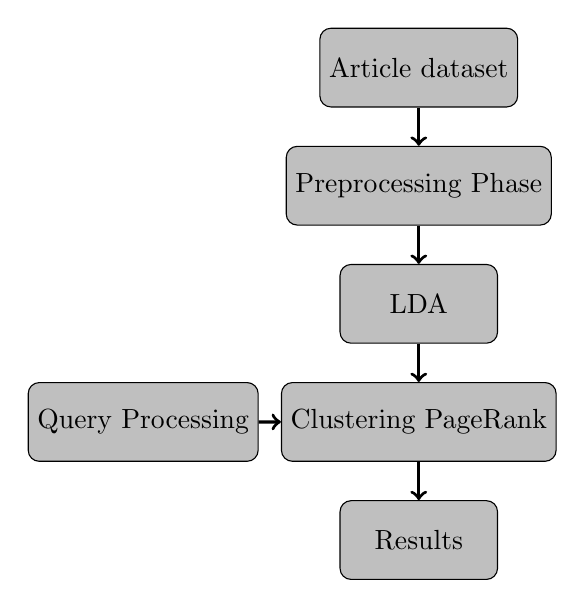
\begin{tikzpicture}[node distance=1.5cm]
    %\draw[step=1cm,gray,very thin] (-8,-8) grid (8,8);
	\node (Dataset) [process] {Article dataset};
	\node (Cleaning)[process, below of=Dataset] {Preprocessing Phase};
	\node (Training) [process, below of=Cleaning] {LDA};
	\node (Cluster PR) [process, below of=Training] {Clustering PageRank};
	\node (Query) at (-3.5, -4.5) [process] {Query Processing};
	\node (Result) [process, below of=Cluster PR] {Results};
	\draw [->, very thick] (Dataset) edge (Cleaning); 
	\draw [->, very thick] (Cleaning) edge (Training);
	\draw [->, very thick] (Training) edge (Cluster PR);
	\draw [->, very thick] (Cluster PR) edge (Result);
	\draw [->, very thick] (Query) edge (Cluster PR);
\end{tikzpicture}
	\caption{Pipeline}
    \label{fig:pipeline}
\end{figure}